\documentclass[a0,portrait]{a0poster}
%%%Load packages
\usepackage{multicol} 			%3-column layout
\usepackage[left=2cm,right=3cm,bottom=-1.2cm,top=0cm]{geometry}			%Reset margins
\usepackage[T1]{fontenc}			%Need for gtamac fonts
\usepackage{textcomp}
\usepackage{mathpazo}			%Load palatino font & pazo math
\usepackage{color}				%Needed for colour boxes & coloured text
\usepackage{amsmath}


%%%Define colours and lengths
\definecolor{headingcol}{rgb}{1,1,1}		%Colour of main title
\definecolor{fillcol}{rgb}{1.0,1.0,1}			%Fill-colour of box
\definecolor{boxcol}{rgb}{0.3,0.5,0.5}		%Edge-colour of box and top banner
\definecolor{author}{rgb}{0.9, 0.9, 0.9}
\fboxsep=1cm							%Padding between box and text
\fboxrule=1mm							%Width of box outline
\renewcommand{\rmdefault}{ppl}			%Reset serif to Palatino
\setlength{\columnsep}{3cm}				%Set spacing between columns
%Uncomment for lines as column separators:
%\setlength{\columnseprule}{1pt}


%%%Format title
\makeatletter							%Needed to include code in main file
\renewcommand\@maketitle{%
\null									%Sets position marker
{
\color{headingcol}\rmfamily\VeryHuge\bf		%Set title font and colour
\vspace{2cm}
\hspace{0.06\textwidth}
\begin{minipage}{0.6\textwidth} 
    \centering
    \@title 
    \par
\end{minipage}
}%
\vskip 0.6em%
\vspace{1cm}
{
\color{author}\rmfamily\LARGE\bf				%Set author font and colour
\hspace{0.14\textwidth}
\begin{minipage}{0.45\textwidth}
    \centering
    \@author
    \par
\end{minipage}}%
\vskip 1cm
\par
\vspace{-7cm}
    % a0 linewidth = 84.1cm
\hspace{2cm}
\vtop{%
    \vskip0pt
    \hbox{%
        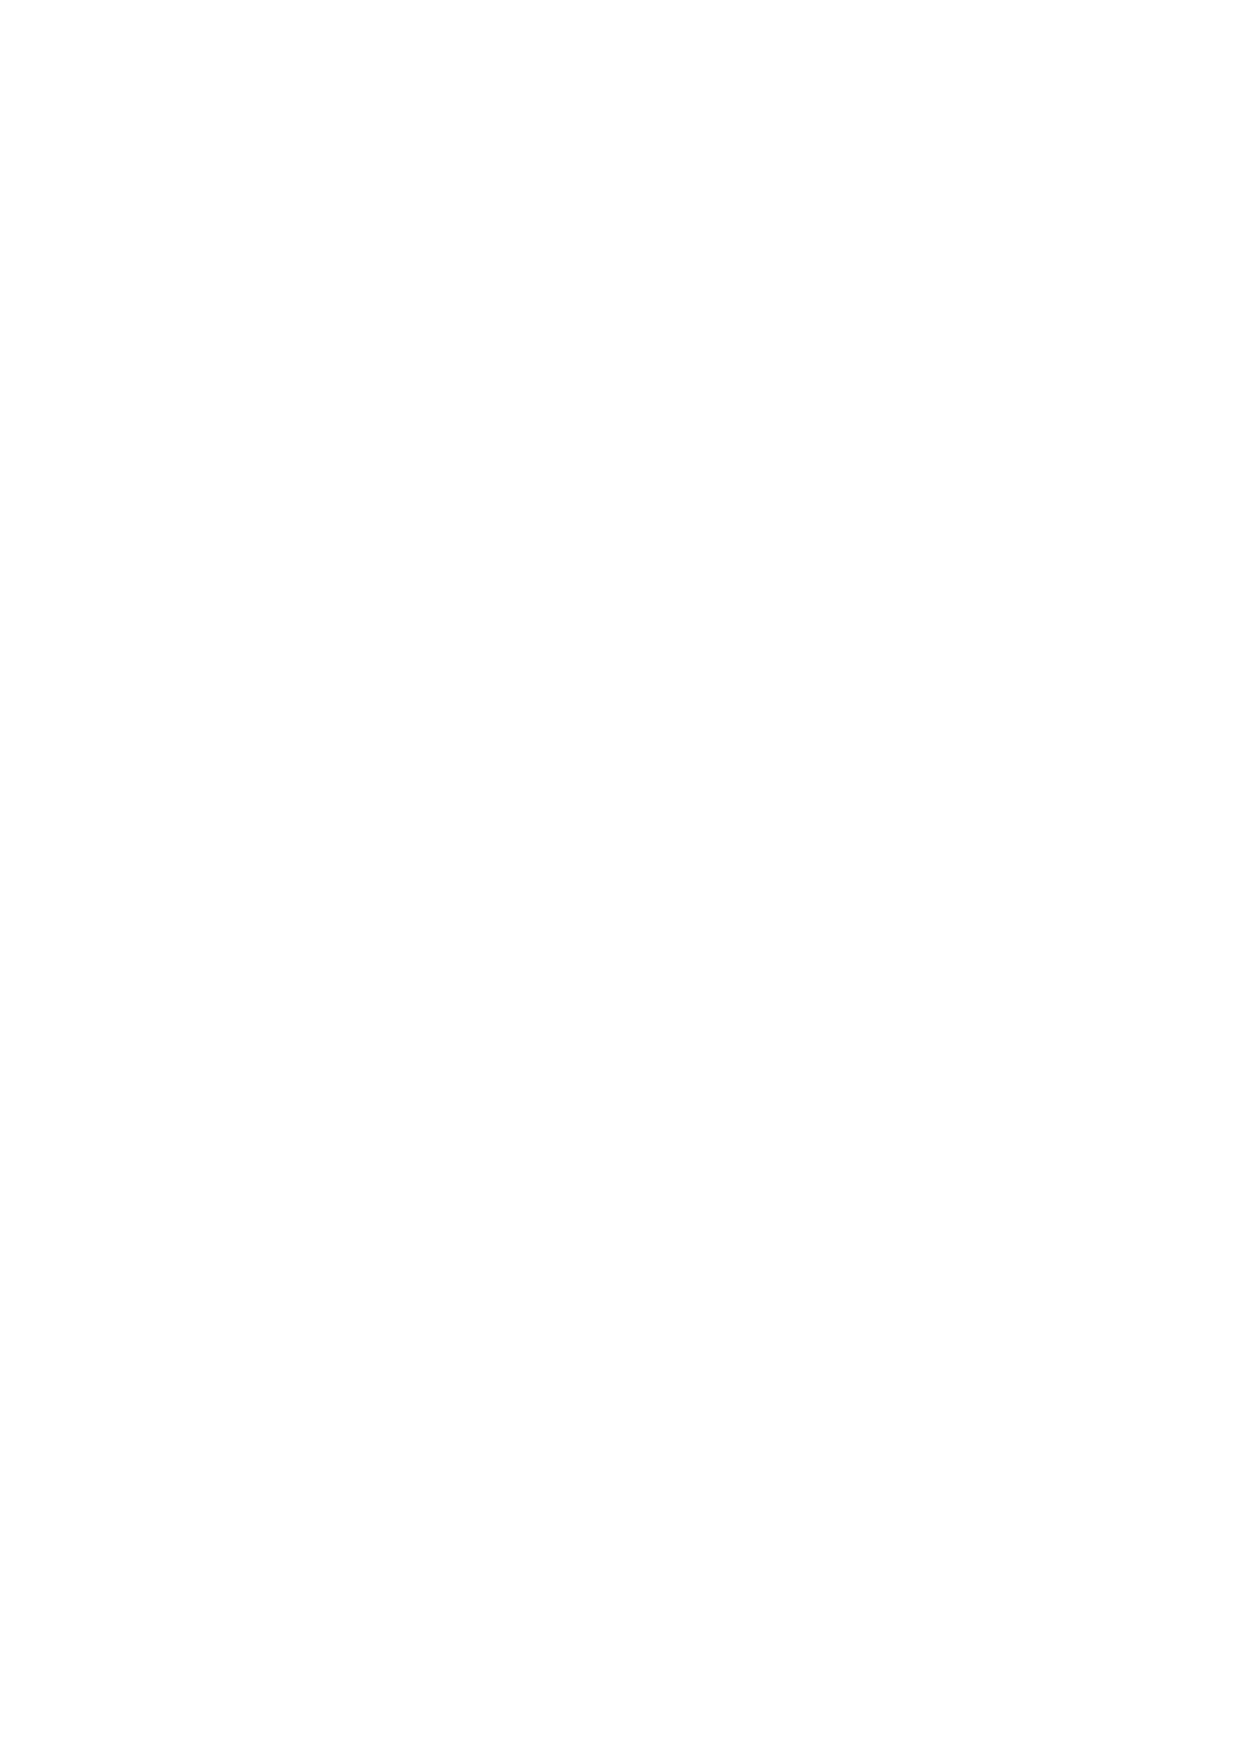
\includegraphics[trim=-0.4cm 0 0 0.5cm, width=20cm]{epsrc_high}
    }%
}
\hspace{47.2cm}
\vtop{%
    \vskip0pt
    \hbox{%
        
\includegraphics[trim=0 0 0 2cm, width=12cm]{kings-logo}
    }%
}
\vspace{1cm}
}
\makeatother

\newsavebox\envbox 					%Define name for boxes used

%%%Define "Section" environment for framed boxes
%%%Usage: \begin{Section}{Name} blah blah blah \end{Section}
\newenvironment{Section}[1]				%Environment takes one argument
%%%Opening
{
\par 
\flushleft
\colorbox{boxcol}{% 						%Draws solid colour box around title
\sffamily\Large\bf\color{headingcol}> \color{white} #1%Typesets section name
\hspace{0.5cm}}
\par\nobreak 
\nointerlineskip 						%Fits title snugly above box (no gap)
\setlength\parskip{-1pt}					%Even snugger
\begin{lrbox}\envbox						%Opens box environment
\begin{minipage}{0.95\columnwidth}		%Opens minipage environment for section contents
}
%%%Closing
{\par
\end{minipage}\end{lrbox}				%Close minipage and box
\fcolorbox{boxcol}{fillcol}{\usebox\envbox}	%Draw box with contents frame colour: boxcol, fill colour: fillcol
\vspace{1cm}							%Add spacing below box
} 
\newenvironment{Section2}[1]				%Environment takes one argument
%%%Opening
{
\par 
\flushleft
\colorbox{boxcol}{% 						%Draws solid colour box around title
\sffamily\Large\bf\color{headingcol}> \color{white} #1%Typesets section name
\hspace{0.5cm}}
\par\nobreak 
\nointerlineskip 						%Fits title snugly above box (no gap)
\setlength\parskip{-1pt}					%Even snugger
\begin{lrbox}\envbox						%Opens box environment
    \begin{minipage}{2.073\columnwidth}		%Opens minipage environment for section contents
}
%%%Closing
{\par
\end{minipage}\end{lrbox}				%Close minipage and box
\fcolorbox{boxcol}{fillcol}{\usebox\envbox}	%Draw box with contents frame colour: boxcol, fill colour: fillcol
\vspace{1cm}							%Add spacing below box
} 
\newenvironment{Section3}
%%%Opening
{
\par 
\flushleft
\par\nobreak 
\nointerlineskip 						%Fits title snugly above box (no gap)
\setlength\parskip{-1pt}					%Even snugger
\begin{lrbox}\envbox						%Opens box environment
    \begin{minipage}{2.04\columnwidth}		%Opens minipage environment for section contents
}
%%%Closing
{\par
\end{minipage}\end{lrbox}				%Close minipage and box
\fcolorbox{boxcol}{fillcol}{\usebox\envbox}	%Draw box with contents frame colour: boxcol, fill colour: fillcol
\vspace{1cm}							%Add spacing below box
} 
\newenvironment{Section4}
%%%Opening
{
\par 
\flushleft
\par\nobreak 
\nointerlineskip 						%Fits title snugly above box (no gap)
\setlength\parskip{-1pt}					%Even snugger
\begin{lrbox}\envbox						%Opens box environment
    \begin{minipage}{0.9843\columnwidth}		%Opens minipage environment for section contents
}
%%%Closing
{\par
\end{minipage}\end{lrbox}				%Close minipage and box
\fcolorbox{boxcol}{fillcol}{\usebox\envbox}	%Draw box with contents frame colour: boxcol, fill colour: fillcol
\vspace{1cm}							%Add spacing below box
} 
\newenvironment{Section5}
%%%Opening
{
\par 
\flushleft
\par\nobreak 
\nointerlineskip 						%Fits title snugly above box (no gap)
\setlength\parskip{-1pt}					%Even snugger
\begin{lrbox}\envbox						%Opens box environment
    \begin{minipage}{0.95\columnwidth}		%Opens minipage environment for section contents
}
%%%Closing
{\par
\end{minipage}\end{lrbox}
\fcolorbox{boxcol}{fillcol}{\usebox\envbox}\hspace{-1.6cm}	%Draw box with contents frame colour: boxcol, fill colour: fillcol
\vspace{1cm}							%Add spacing below box
} 
\usepackage{physics}
\usepackage{graphicx}
\graphicspath{ {images/} }
\usepackage{caption}
\usepackage{array}
\usepackage{wrapfig}
 

\title{Dissipative Control of Quantum Dynamics from Biased Trajectory Ensembles}

\author{Fergus Barratt (fergus.barratt@kcl.ac.uk) \\Supervisors: Andrew Green \& Peter Sollich}

\begin{document}
\pagenumbering{gobble}

\hspace{-4.1cm}								%Align with edge of page, not margin
\colorbox{boxcol}{		
\begin{minipage}{1189mm}					%Minipage for title contents
%\vspace{-13cm}							%Shift up over header image
\maketitle
\end{minipage}}
\vspace{1cm}

\begin{multicols}{3}							%Use 3-column layout
\raggedcolumns							%Don't stretch contents vertically
\Large

%%%Column1
\begin{Section}{I: Introduction}
\begin{itemize}
    \item Technological potential of quantum\\ systems due to state space scaling.
    \item Environmental decoupling a challenge to effective use of quantum technology i.e.\ in adiabatic quantum computation 
    \item New tools from statistical mechanics?
\end{itemize}
\vspace{0.75cm}
\end{Section}

\begin{Section}{1: Trajectory Ensembles}
    \begin{itemize}
    \itemsep1cm
        \item Ensembles of trajectories - like thermal ensembles. Partition function:~\cite{Garrahan2007}
            \begin{equation}
                \mathcal{Z}_A(s, t) = \sum_A \Omega_{dyn}(A, t)e^{-sA}\nonumber
            \end{equation}

        \item Markovian, paths biased (like canonical ensemble) by time extensive observable A (E) with strength s ($\beta$). $\mathbb{W} \rightarrow \mathbb{W}_A$ in
            \begin{equation}
                \pdv{\vec{P}_A}{t} = \mathbb{W}_A(s) \vec{P}_A,\nonumber
            \end{equation}
            leads to
            \begin{equation}
                \mathcal{Z}_A(s, t) \sim e^{t \psi_A(s)}\nonumber
            \end{equation}
            with $\psi_A(s)$ largest eigenvalue of $\mathbb{W}_A(s)$: \emph{dynamical free energy}.
    \item Singularities in dynamical free energy $\rightarrow$ \emph{dynamical phase transitions}: different dynamical behaviour i.e.\ transition to chaos, jamming in glasses
    \item Dynamical phase transitions studied in \emph{kinetically constrained models} (KCMS) of glass formers (fig.~\ref{fig:KCM})
\end{itemize}
    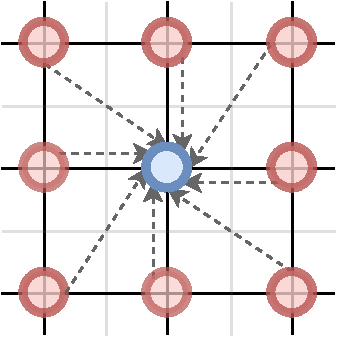
\includegraphics[width=\linewidth]{kcm}
    \captionof{figure}{Schematic of site of Kinetically Constrained Model. Site $i$ (blue) transitions from $n_i \rightarrow 1-n_i$ with rate $W(n_i \rightarrow 1-n_i) = C(\{n_j\}) \frac{e^{\beta(n_i-1)}}{1+e^{-\beta}}$, where $C(\{n_j\})$ is a function only of the values of sites $n_j$ (red)} \label{fig:KCM}
\end{Section}

\columnbreak

%%%Column 2

\begin{Section2}{II: Aims}
    \begin{itemize}
        \item Classical glasses $\rightarrow$ KCMs\\
        $\rightarrow$ \emph{biased trajectory ensembles}\cite{Garrahan2007}
        \item Keldysh theory $\rightarrow$ dissipation \\
            $\rightarrow$ analogy to bias in trajectory ensembles
        \item Transition from quantum resources to \\
            absence as \emph{dynamical phase transition}
    \end{itemize}
            \vspace{-11cm}\flushright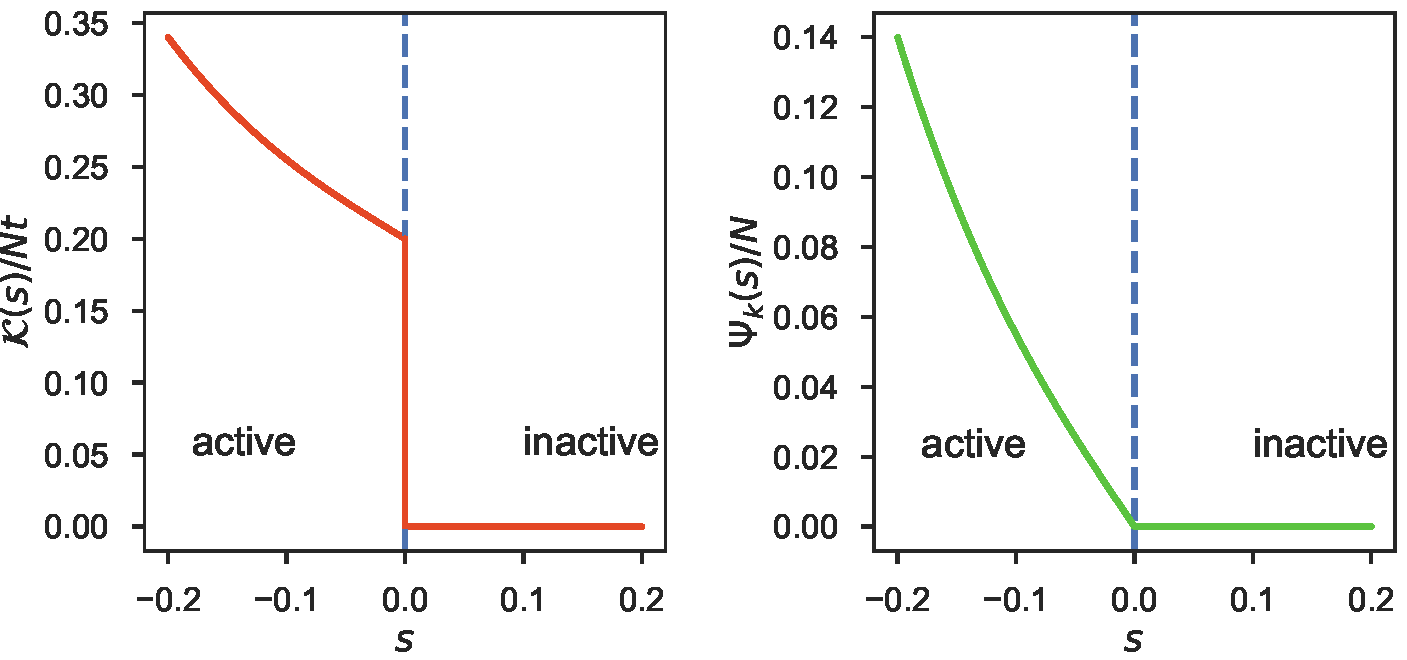
\includegraphics[width=0.5\linewidth]{dyn_phase_transition}\flushleft
            \vspace{-1cm}
            % \captionof{figure}{Dynamical phase transition}

\end{Section2}

\vspace{0.544cm}
\begin{Section}{2: Matrix Product States}

\begin{itemize}
    \itemsep1cm
    \item Interesting bit of most Hilbert spaces small, permits efficient numerics
\end{itemize}
\vspace{0.5cm}
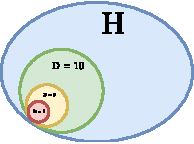
\includegraphics[width=\linewidth]{D}
\begin{itemize}
    \itemsep1cm
    \item Many-body quantum state 
\begin{equation}
    \ket{\psi} = \sum_{\sigma_1, \ldots, \sigma_L} C_{\sigma_1, \ldots, \sigma_L} \ket{\sigma_1, \ldots, \sigma_L}, \nonumber
\end{equation}
\item MPS decomposition ($\Lambda$ diagonal)
    \begin{equation} \ket{\psi} = \sum_{\sigma_1, \ldots, \sigma_L} \Gamma^{\sigma_1}\Lambda_1 \ldots \Lambda_{L-1}\Gamma^{\sigma_L} \ket{\sigma_1, \ldots, \sigma_L }\nonumber
    \end{equation}
    \item Important bit of Hilbert space spanned by MPS with $\Lambda$ truncated to D dims
    \item D grows with time evolution. Project back to D subspace - classical EOM
\end{itemize}
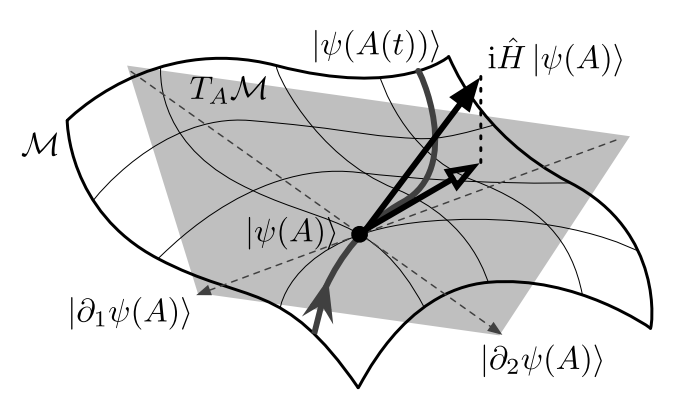
\includegraphics[width=\linewidth]{tdvp}
\captionof{figure}{Time-dependent variational principle~\cite{Haegeman2011}}
\end{Section}

\begin{Section5}
\begin{minipage}{1\linewidth}
    \vspace{0.2cm}
    \centering
    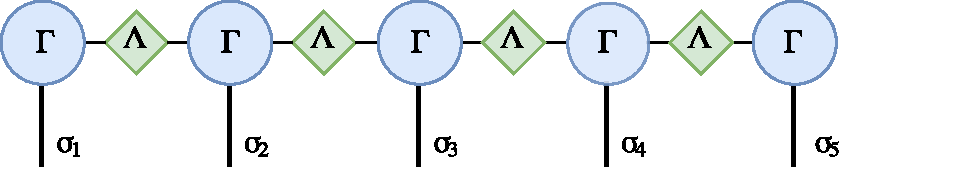
\includegraphics[width=1.15\linewidth]{mps}
 \captionof{figure}{5-site Open Boundary Condition MPS}
\end{minipage}
\end{Section5}
\columnbreak

%%%Column 3

\flushleft\fcolorbox{white}{fillcol}{\usebox\envbox}
\vspace{14.32cm}
\begin{Section}{3: Non-Equilibrium QFT: Keldysh}

        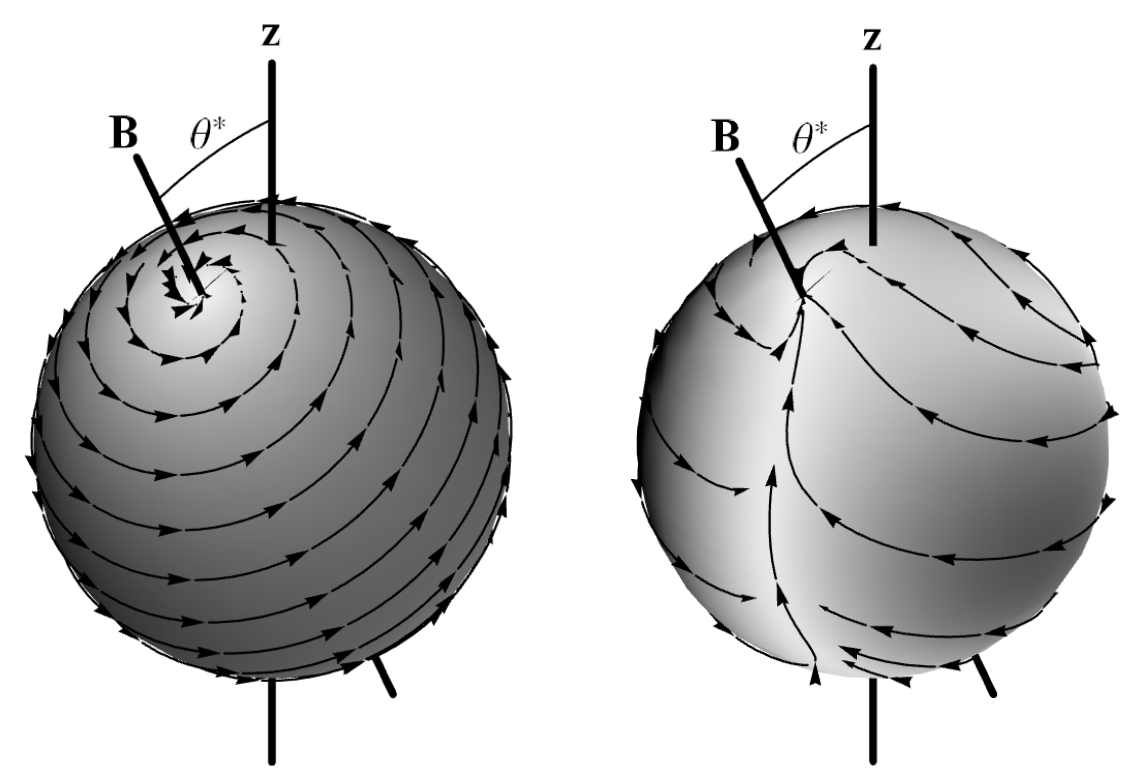
\includegraphics[width=\linewidth]{spins1}
        \captionof{figure}{Different dynamical behaviour~\cite{Crowley2016}}
        \vspace{0.15cm}

\begin{itemize}
    \itemsep1cm
    \item Evolve the state forward in time $(-\infty \rightarrow \infty)$, rewind $\infty \rightarrow -\infty$: fig.~\ref{fig:keldysh}
    \item Separate fields on forward and backwards contours ($\phi^+, \phi^-$)
    \item Constructing the path integral $\rightarrow$ redundancy in the Green's Functions.
    \item Combinations such that $\ev{\phi^{cl}\phi^{cl}}$ = 0
        \begin{equation}
            \phi^q = \phi^+ - \phi^- \qquad \phi^{cl} = \phi^+-\phi^- \nonumber
        \end{equation}
    \item Introduce a bath interacting with system, integrate out bath, generate semi-classical path integrals for quantum systems  
    \item Classical average over delta function $\rightarrow$ MSRJD formalism
        \begin{equation}
            \ev{\delta\left(\dot{x}(t) - f(x) - \xi(t)\right)} \nonumber
        \end{equation}
    \item Distribution over paths. Connected to the classical trajectory ensemble?
\end{itemize}


\end{Section}
\begin{Section5}
\begin{minipage}{1\linewidth}
    \vspace{0.2cm}
    \centering
    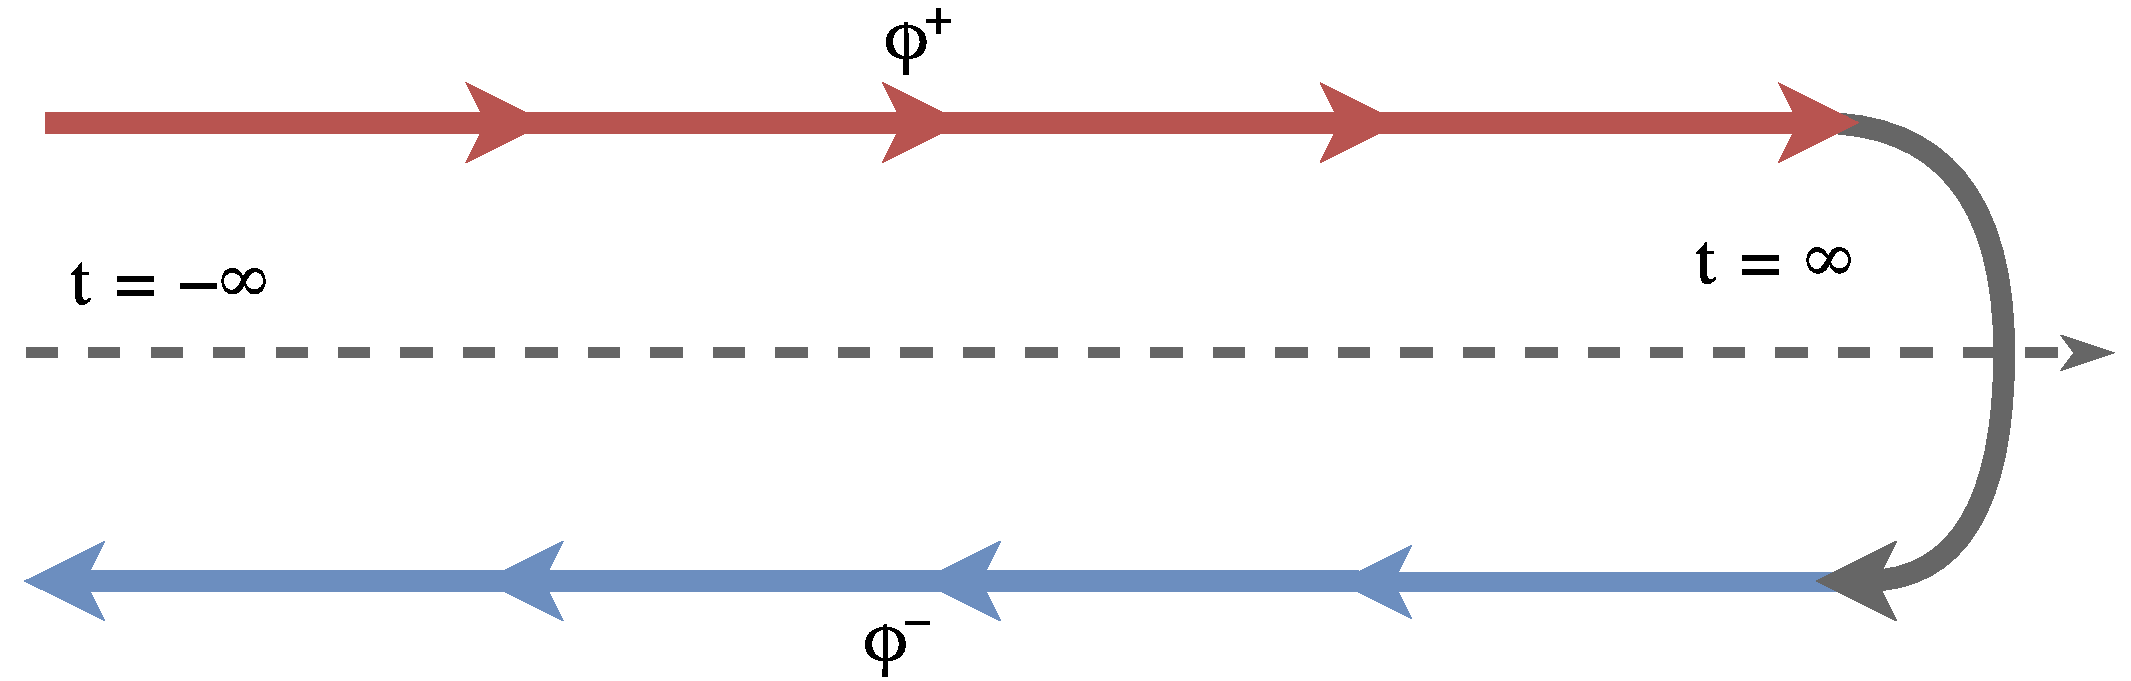
\includegraphics[width=1.03\linewidth]{keldysh}
        \captionof{figure}{Keldysh Contour}\label{fig:keldysh}
\end{minipage}
\end{Section5}
%\bibliographystyle{plain}
%\bibliography{halobib}

\end{multicols}
%%%Closing

\vspace{-5.5cm}
    \flushright

\vfill
\flushleft
    \bibliography{ref}{}
    \bibliographystyle{abbrv}
    \vspace{2.5cm}
\end{document}
